\documentclass{article}
\usepackage{amsmath,amssymb,indentfirst,epsfig,ifthen,booktabs,color,multirow,float,nomencl,lineno}
\modulolinenumbers[5]
%\usepackage[figure]{hypcap}
\makenomenclature

\renewcommand{\nomgroup}[1]{%
%\ifthenelse{\equal{#1}{A}}{\item[\textbf{Roman Symbols}]}{%
\ifthenelse{\equal{#1}{G}}{\item[\textbf{Greek Symbols}]}{%
\ifthenelse{\equal{#1}{C}}{\item[\textbf{Abbreviations}]}{%
\ifthenelse{\equal{#1}{S}}{\item[\textbf{Subscripts}]}% matches mathematical symbols
}% matches Subscripts
}% matches Abbreviations
}% matches Greek Symbols
}% matches Roman Symbols

\makeindex
\begin{document}

\title{A multi-stage heating system for solar parabolic trough power plants}
\date{}
\author{}
\maketitle

\begin{abstract}
In a traditional solar parabolic trough power plant, the potential of exergy loss reduction in the heating process of Rankine cycle is large. There exist large temperature differences between the heat transfer fluid (HTF) and water in the steam generator subsystem (SGSS). In order to reduce the temperature differences, this paper put forward a novel multi-stage heating system (MSHS) with different HTF flows to lower the required HTF temperature. A flow control strategy of HTF depending on the analytical system model was derived. Energy and exergy efficiency of the MSHS was analyzed and compared with the SGSS of traditional solar parabolic trough power plant. Result shows that the MERS can effectively decrease the exergy loss in the heating process, thus the performance of the plant can be improved.
\end{abstract}

\noindent{\bf Keywords: }multi-stage heating system, exergy-loss reduction, solar parabolic trough, heat transfer fluid
\newpage{}

\linenumbers

\section{Introduction}

Solar energy, which has the advantages of widely distribution, huge amount, inexhaustible and no pollution, has received much attention by many countries and been regarded as the best potential candidate of the fossil energy.~\cite{Guo2016,Salgado2017}
Concentrated solar power (CSP) is a technology uses mirrors or lenses to concentrate sunlight onto a receiver that absorbs solar energy and transfer it to a heat transfer fluid (HTF) such as a synthetic oil, molten salt or air. The HTF then directly or indirectly used as the heat source in a power cycle.
Parabolic trough is the most mature and commercially deployed CSP technology.

Most of commercial and pilot parabolic trough power plants use oil as heat transfer fluid, such as SEGS and Anddasol.~\cite{Price2002,Liu2016}

1. Need to reduce the temperature difference between HTF and water

2. What's other's work?

3. Our work

In a solar parabolic trough power plant in which intermediate heat-transfer fluid (take oil for instance) is used, heat addition to the working fluid (take water for instance) takes place in three counterflow heat exchangers (steam generator subsystem, SGSS) as shown in \ref{fig:PTC}. The SGSS consists of preheater, evaporator and superheater. The flow rates of both oil and water remain the same in the three heat exchangers.~\cite{Rovira2011}
The water has phase change in the three heat exchangers, from liquid to vapor in the evaporator, however, oil remains liquid. The heat capacity of water in each heat exchanger  differs significantly. The heat capacity of oil has no significant difference since no phase change. The heat transfer process is illustrated on \ref{fig:DeltaTmin}. Large temperature differences exist at the inlets and outlets of the heat exchangers, which leads to large entropy production during the entire heat exchange process.

\begin{figure}[htbp]
\centering
	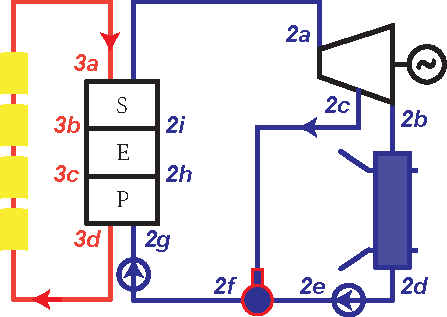
\includegraphics[width = 0.4\columnwidth]{fig/PTC}
	\caption{A typical solar parabolic trough system}
	\label{fig:PTC}
\end{figure}
\begin{figure}[htbp]
\centering
	\includegraphics[width = 0.5\columnwidth]{fig/DeltaTmin}
	\caption{The steam generating process in counterflow heat exchangers}
	\label{fig:DeltaTmin}
\end{figure}

%Electricity, the most common energy source, is still dominantly generated from fossil fuel combustion, which not only has a limited life but also produces pollution. The increasing problems of environmental pollution and energy security have strengthened interest in clean and sustainable energy. Solar energy, a clean, safe, inexhaustible, widely distributed energy, has received much attention as the most promising candidate to substitute for the conventional fossil fuels for electricity supply. 

The problems of environmental pollution and energy security have strengthened interest in solar energy for it's advantages of clean, safe, inexhaustible, widely distributed. Solar thermal power generation, for its good compatibility on the existing fossil fuel power plants, has received much attention as the most promising candidate to substitute for the conventional fossil fuels for electricity supply. There exists several kinds of solar thermal power technologies, including parabolic trough, power tower and dish/engine, among which parabolic trough power is the most commercial applied for its low cost. However, the power generation efficiency of the parabolic trough power plant is also relatively low. Many efforts are focused on the research and technology of increasing the power generation efficiency.

Solar parabolic trough, the most commercial utilized solar thermal power generation form, uses heat transfer fluid (HTF, usually oil or salt) to run trough the receiver to absorb the heat generated by the concentrated sunlight. The HTF is then used to heat the working fluid of Rankine cycle (usually water) from sub-cooling water to superheated steam in the steam generator subsystem (SGSS).

%In a traditional solar parabolic trough system, HTF runs through the receiver to collect the heat produced by the converged sunlight. Then the HTF is used to heat the working fluid of Rankine cycle in the heating system. The working fluid is usually water or organic fluid, this paper takes water as illustration. 

\begin{figure}[htbp]
\begin{center}
	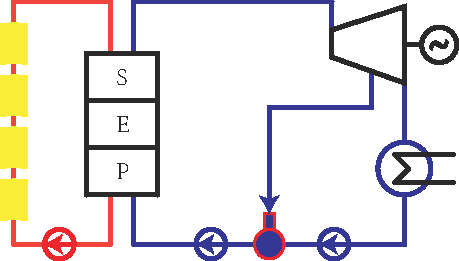
\includegraphics[width = 0.7\columnwidth]{fig/SPTS}
	\caption{Schematic layout of a solar parabolic trough system}
	\label{fig:spts}
\end{center}
\end{figure}

As a conclusion, SEA of serial flows with reverse order always has the best performance and adaptability under different parameters. Given heating and cooling fluids, using serial flow with reverse order is always a best choice.



\clearpage
\printnomenclature[2.5cm]{}
\clearpage

\bibliography{MSHS}
\bibliographystyle{unsrt}

\end{document}

